% document type
\documentclass[12pt]{article}

% packages
\usepackage[total={170mm,230mm}]{geometry}
\usepackage[utf8]{inputenc}
\usepackage[T1]{fontenc}
\usepackage[russian]{babel}
\usepackage{graphicx}
\usepackage{amssymb}
\usepackage{amsfonts}
\usepackage{amsmath}
\usepackage{amsthm}
\usepackage{physics}
\usepackage{nicefrac}
\usepackage{cancel}
\usepackage{hyperref}
\usepackage{cmap}

\title{Лабораторная работа}
\author{Александр Козлов}

\begin{document}
\maketitle

\section{Кольца Ньютона}
\subsection{Определение масштабного коэффициента}
Для определения масштабный коэффициент определим сколько пикселей в одном миллиметре. Будем работать со шкалой, представленной на рисунке \ref{fig:1}. 
\begin{figure}[htbp]
	\centering
	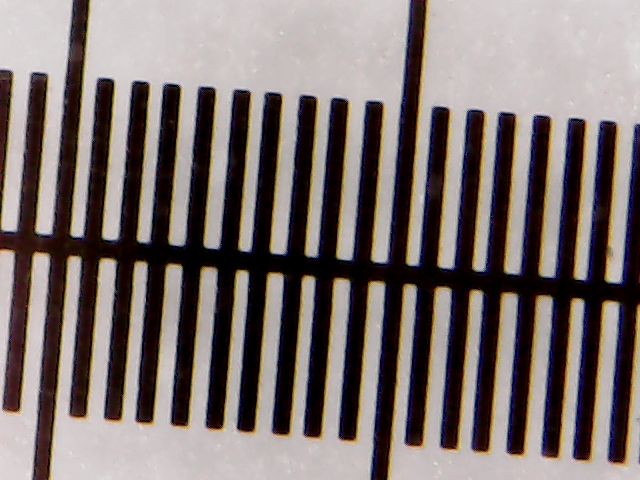
\includegraphics[width = 0.5\linewidth]{../data/1-0.jpg}
	\caption{Нониусная шкала колибратора. Между двумя соседними маленькими отметками лежит одна десятая часть миллиметра. Ось шкалы находится под углом $5^\circ$ к горизонту.}
	\label{fig:1}
\end{figure}
В 12 сверху строке пикселей имеется картина интенсивностей, изображённая на рисунке \ref{fig:2}, откуда можно определить расстояние между двумя большими чёрными праллельными полосами.
\begin{figure}[htbp]
	\centering
	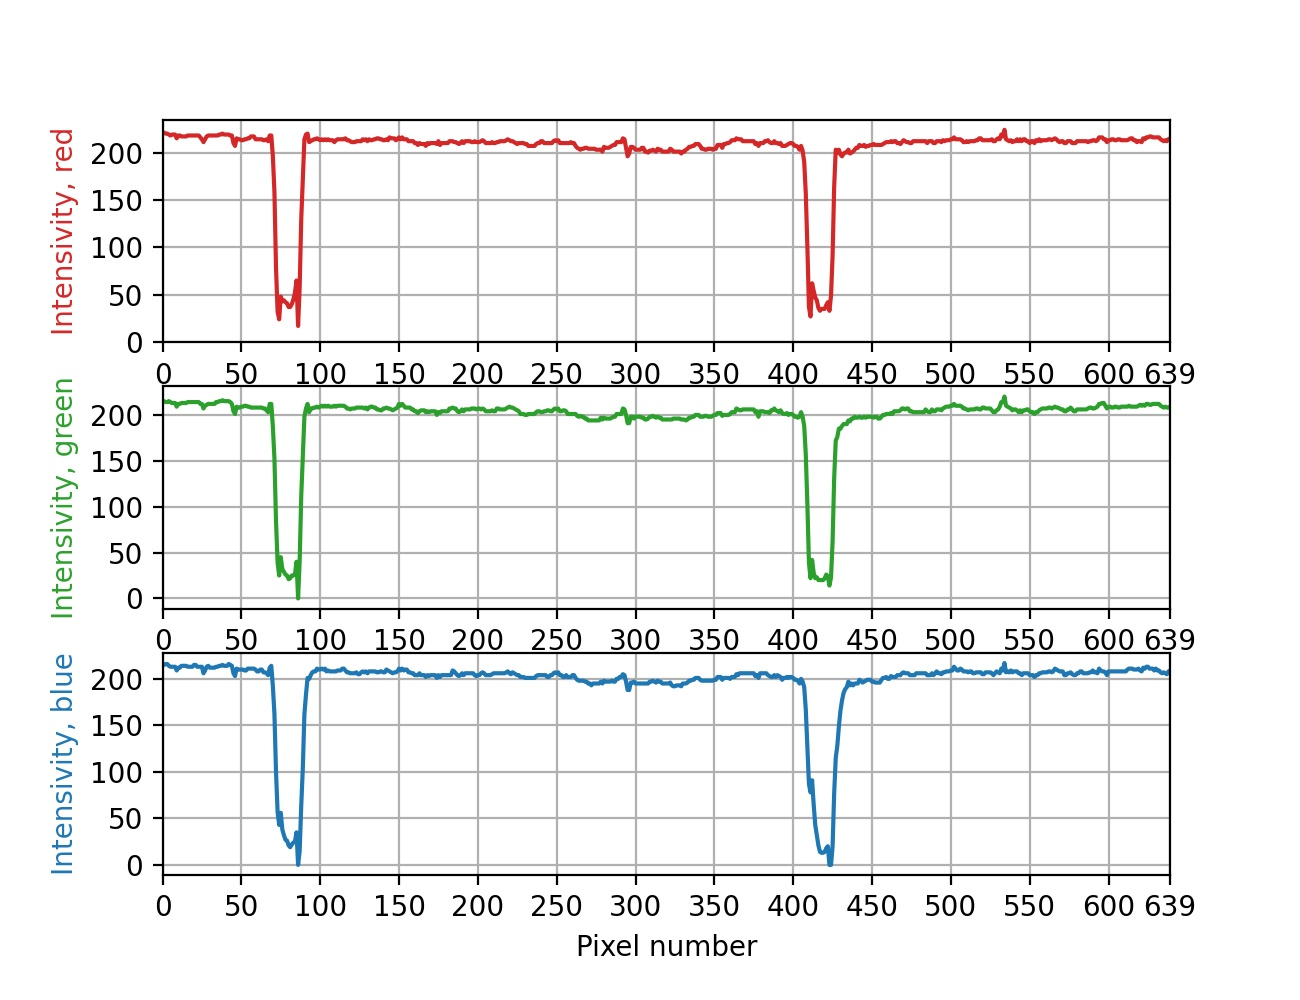
\includegraphics[scale = 1]{../plots/1-0.jpg}
	\caption{Интенсивность пикселей в 12 строке сверху изображения \ref{fig:1}.}
	\label{fig:2}
\end{figure}
Результаты таких измерений занесены в таблицу \ref{tab:1}. Точность определения положений примем равной $10$ пикселям (так как ширина углублений на графиках интенсивностей составляется пимерно $20$ пикселей). Тогда точность определения расстояний составит $20$ пикселей. Усреднённое по цветам расстояние между длинными черными полосами будет равно $338\pm20$ пикселей. 
\par Но стоит так же учесть наклон оси шкалы к горизонту (тут под горизонтом понимается горизонтальная ось), который составляет $5^\circ\pm0.25^\circ$. Из элементарных геометрических соображений ясно, что нужно умножить определённое ранее расстояние на косинус угла наклона. Тогда получим, что правильное расстояние между двумя длинными полосами составляет $333\pm20$ пикселей. 
\begin{table}
\centering
\caption{\label{tab:1}Результаты измерений расстояний между черными длинными полосами для различных цветов.}
\begin{tabular}{|l|l|l|l|} 
\hline
Цвет    & \begin{tabular}[c]{@{}l@{}}Положение\\левой полосы,\\пиксели\end{tabular} & \begin{tabular}[c]{@{}l@{}}Положение\\правой полосы,\\пиксели\end{tabular} & \begin{tabular}[c]{@{}l@{}}Расстояние между\\двумя черными полосами, \\пиксели\end{tabular}  \\ 
\hline
Красный & 80                                                                        & 416                                                                        & 336                                                                                          \\ 
\hline
Зелёный & 80                                                                        & 417                                                                        & 337                                                                                          \\ 
\hline
Синий   & 80                                                                        & 420                                                                        & 340                                                                                          \\
\hline
\end{tabular}
\end{table}
Здесь для вычисления погрешности использовалась формула
\begin{equation}
	\dd l_{new} = \dd \qty(l_{old}\cdot\cos{\theta}) = \dd l_{old} \cdot \cos{\theta} + l_{old} \cdot \sin{\theta} \cdot \dd \theta,
\end{equation}
где угол $\theta$ выражен в радианах. Таким образом, $1$ мм соответствует $333\pm20$ пикселей, значит, масштабный коэффициент будет равен
\begin{equation}
	k = 3 \dfrac{\text{мкм}}{\text{пиксель}}.
\end{equation}
Погрешность будет равна примерно $0$, ибо согласно формуле для погрешности
\begin{equation}
	\dd \dfrac1l = \dfrac{\dd l}{l^2} = 0.12\ {\text{пиксель}}^{-1}
\end{equation}
она получается мала и при окгруглении до значящих порядков становится равной нулю.


\end{document}